\documentclass[12pt, letterpaper, twoside]{article}
\usepackage[utf8]{inputenc}
\usepackage{dirtytalk}
\usepackage{graphicx}
\usepackage{amssymb}
\usepackage[backend=biber,style=numeric, natbib=true, sorting=none, maxbibnames=13, url=false]{biblatex}
\addbibresource{ge-refs.bib}


	
\title{Linking amino acid sequences to sources and fates of organic matter in aquatic systems}
\author{Megan Duffy}
\date{April 21, 2020}

\begin{document}
	
	\begin{titlepage}
		
		\maketitle
		\begin{center}
			A description of proposed Ph.D. dissertation research \\
			\bigskip
			\bigskip
			Supervisory committee \\
			\bigskip
			Rick Keil (chair) 
			
			Jeff Richey 
			
			Gabrielle Rocap 
			
			Anitra Ingalls 
			
			Sarah Stroup (GSR)
		\end{center}
		
	\end{titlepage}
	

\newpage

\tableofcontents{}

\newpage

\section*{Overview}

Proteins enact life’s intent: directed by genes and informed by the environment, these macromolecules are the engines that power the cells of all biological entities on Earth. From viruses and bacteria to humans and blue whales, proteins serve a vast range of metabolic, transport, communication, and structural purposes. Life, in turn, along with geological and chemical drivers, modulates the planetary cycles of carbon, oxygen, and nitrogen.

By unlocking the information stored in peptide and protein sequences, we can learn the biological origins and functions of cells within a community. For organic geochemists, there is useful information here as well: proteins make up a large proportion of organic carbon and nitrogen in aquatic systems. Thus, the cycling and degradation dynamic of proteins is of great importance when thinking about global organic carbon preservation and sequestration. 

\textbf{My proposed Ph.D. research addresses the cycling of proteins and protein-derived organic matter in both laboratory settings and environmental systems.} Chapter 1, my M.S. project, describes the usefulness of integrating a different kind of peptide sequencing, \textit{de novo} sequencing, into the traditional environmental proteomics workflow in order to access degraded and unanticipated sequences. This is described in \say{Protein cycling in the eastern tropical North Pacific oxygen deficient zone: a \textit{de novo}-assisted peptidomic approach}, [Duffy et al., \textit{in review}]. The three subsequent projects utilize this technique to ask questions about proteins and peptide cycling in complex environmental systems. 

Chapter 2 uses the \textit{de novo}-assisted peptidomic technique to follow the peptides of a diatom through a simulated bloom and subsequent degradation by a natural microbial community. Chapter 3 is a peptidomic-based comparison of organic matter across seasons, stations (on and offshore) and sinking class of marine organic matter in an ODZ. Chapter 4 moves out of the purely marine realm and bridges the span between terrestrial and marine systems in the Amazon River-Atlantic continuum, probing how organic matter travels from land to sea, and how microbes alter its reactivity and character.

\newpage

\section{Proposed work}

\subsection{{Chapter 1: De novo}-assisted peptidomics helps in the study of marine carbon flux and protein degradation}

\textit{Note}: The work comprising Chapter 1 is detailed in a submitted manuscript sent to all committee members, and as such will not be fully introduced here. 

Developments in high resolution mass spectrometry and computing have facilitated metaproteomic investigations of proteins in suspended \cite{dong_characterization_2010, bridoux_suspended_2015, bergauer_organic_2017} and sinking \cite{moore_identifying_2012} organic matter. These powerful metaproteomic tools could help resolve questions about protein and peptide degradation in the ocean, but they are currently limited in that they are designed to identify intact proteins from living cells.

Current metaproteomic workflows adhere to a bottom-up proteomic approach that relies on peptide-spectrum matching through database searching \cite{saito_progress_2019}, with databases derived from  complementary metagenomic or metatranscriptomic analyses and/or publicly available sequence data. This approach has limitations for protein in environmental organic matter, a complex mixture of living, dead, and degraded material. Deviations from a protein's DNA blueprint, post-translational modifications (PTM), occur as a result of that protein’s intended biochemical function and also through degradative processes \cite{kim_methionine_2014} that are poorly understand. Indeed, it is typical that fewer than half of all tandem mass spectra acquired in shotgun proteomics experiments are successfully matched to a peptide from a database \cite{chick_mass-tolerant_2015}. 

\textit{De novo} sequencing is a database-independent tool that uses the same tandem mass spectral information as a peptide-spectrum matching analysis. Rather than comparing peptides to a protein database, first principles-based algorithms are used to establish sequences directly. Several styles of \textit{de novo} sequencing algorithms exist, but all use respective mass differences between fragment ion peaks to piece back together the original peptide ion amino acid sequence.  While the original method of protein sequencing, \textit{de novo} is now mainly used in antibody peptide sequencing (i.e., only when a database-derived sequence is unavailable). This is because \textit{de novo} sequencing is generally less accurate than database searching, often because of insufficient mass accuracy \cite{muth_navigating_2015} or uneven fragmentation patterns in tandem mass spectrometry \cite{lu_algorithms_2004}. But analogous to antibody peptides, degraded peptides are inherent unknowns in the environment. They are difficult to predict or make a database entry for, but surely are present and highly relevant to organic matter cycling. 

\subsubsection{Benchmark: \textit{Prochlorococcus marinus} culture}

As a benchmark study, I compared the sequencing performance of a well-established \textit{de novo} algorithm against traditional database searching on a high resolution mass spectrometry (HRMS) dataset from a \textit{Prochlorococcus marinus} culture. \textit{P. marinus}, a ubiquitous free-living marine cyanobacterium found throughout the world’s oceans \cite{chisholm_novel_1988}, was an advantageous marine microbe for this assessment given its small and relatively well-characterized proteomes \cite{paul_distinct_2010}.

\begin{figure}
	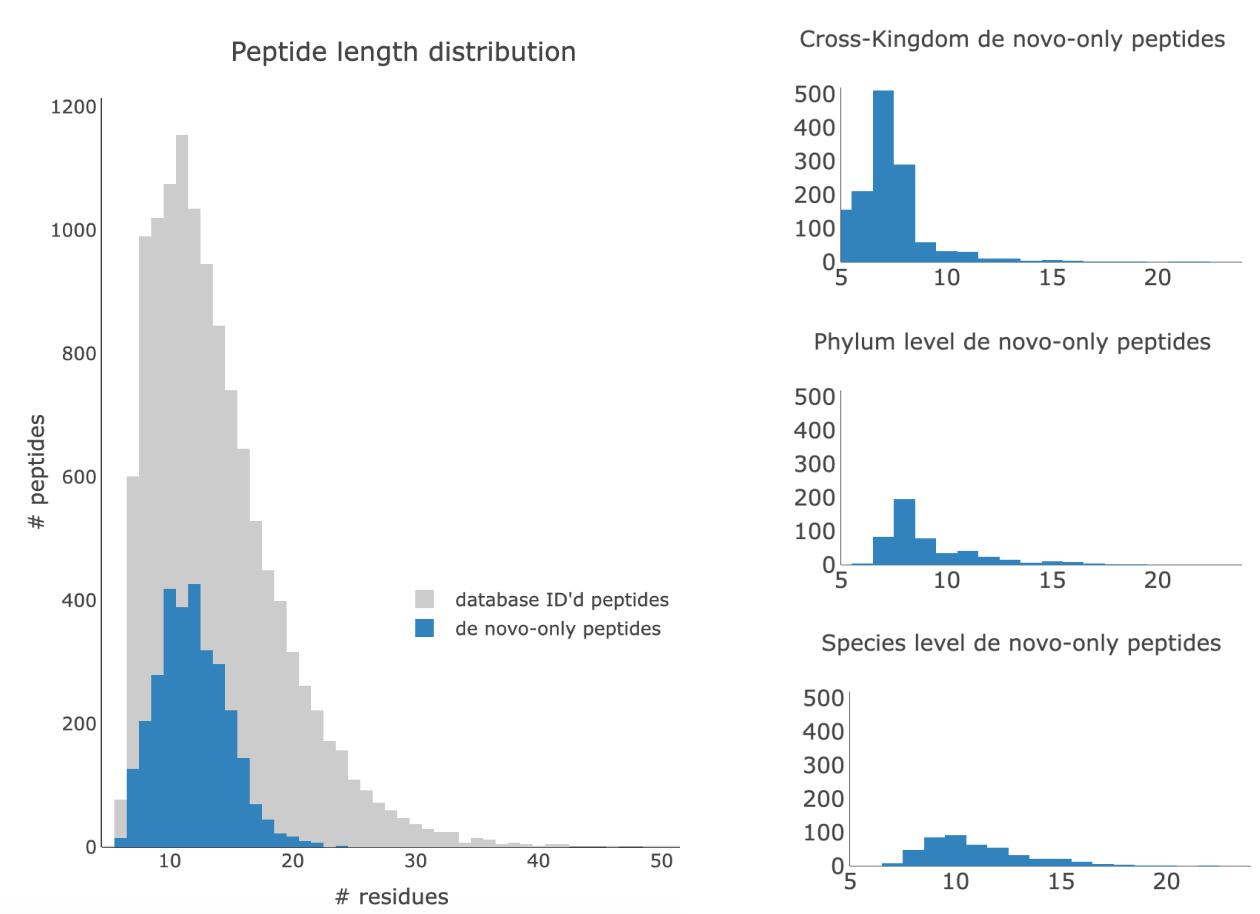
\includegraphics[width=\linewidth]{fig1-denovo.jpg}
	\caption{Histograms showing a) overlaid distributions of sequenced peptide lengths (number of amino acid residues) for database search-identified (grey) and \textit{de novo}-only peptides (blue) of cultured \textit{Prochlorococcus marinus} MED4 protein LC-MS/MS dataset. Of 12,160 database peptides, the mean length was 13.8 residues; of 3,019 \textit{de novo} peptides, the mean length was 10.9 amino acids. Distributions of \textit{de novo}-only peptide lengths for individual taxonomic rankings are shown for b) cross-kingdom, c) phylum, and d) species.}
	\label{fig:de-novo-hists}
\end{figure}

I performed \textit{de novo} peptide sequencing with a commercially available algorithm (Peaks \cite{ma_peaks:_2003}) and database searching, aligning and comparing the two resulting groups of peptides by several criteria: coverage of the known \textit{Prochlororoccus} proteome, degree and types of mass modification, length (number of amino acids), and taxonomic specificity (the degree to which a certain peptide is identifying of and unique to one organism's protein sequence or many across different taxa.)

The \textit{de novo} algorithm did find peptides unidentified through database searching that boosted the overall protein identifications by 6\%. \textit{De novo} peptides were, on average, almost 3 residues shorter than the average of the database-identified peptides [Figure \ref{fig:de-novo-hists}]. Peptide length is an important metric in an metaproteomic context because with increased amino acid space, peptide sequences have more potential to be specific to a particular parent protein. 

To establish the specificity of \textit{de novo}-only sequences (\textit{de novo} sequences that did not align with database-ID'd peptides), I interrogated their sequences against the UniProt Knowledgebase (UniProtKB) protein database using Unipept, a tool designed for tryptic peptide sorting and identification. Unipept uses a lowest common ancestor (LCA) approach to match peptides to as low a resolved taxonomic identification level as is possible given the input sequence. I found that many \textit{de novo}-only peptides are taxonomically specific, with 17\% specific to at least the phylum Cyanobacteria, and 15\% specific to the species level [Figure \ref{fig:de-novo-hists}]. In contrast, of the database-identified peptides; 51\% of peptides matched to the species level. Overall, this comparison showed that the \textit{de novo}-only peptides sequenced from the \textit{Prochlorococcus} culture data are not as specific to their organismal source to those sequenced by traditional database searching, but still have potential to identify individual organisms in a mixed community.  It is important to note that the \textit{de novo}-only non-specific peptides, while not taxon-identifying, nevertheless represent valuable information, especially if one is less concerned about organismal source and wishes to evaluate sequence similarity with respect to preservation and degradation.  

I searched for 30 different mass modifications, and the seven most commonly observed in this dataset were carbamidomethylation (on cysteine), oxidation (on methionine), acetylation, formylation, deamidation (on asparagine and glutamine), dehydration and phosphorylation. Since carbamidomethylation is performed during experimental peptide preparation and set during both database and \textit{de novo} searches, I expect no difference in levels of this modification been the peptide pools. Indeed, no significant difference in carbamidomethylation is observed between database and \textit{de novo}-only peptides. However, in the case of every other modification I searched for, the \textit{de novo}-only peptides are more modified - by up to 10\% more in the case of acetylation and to lesser extents for oxidation, formylation, deamidation, dehydration, and phosphorylation. 

Thus, the culture study shows that while the results of \textit{de novo} searches are not as comprehensive in coverage as the database approach, \textit{de novo} sequencing does complement the database search by a) identifying peptides that wouldn’t otherwise have been discovered, b) identifying peptides that have been post-translationally modified, and c) providing output of non-specific peptides for further evaluation. 

\subsubsection{Preliminary environmental application: the eastern tropical North Pacific}

The exciting application of \textit{de novo} peptide sequencing is to uncharacterized systems, exemplified by the challenges of marine environments. In this preliminary study as part of my M.S. work, I evaluated six POM samples from the eastern tropical North Pacific (ETNP) oxygen deficient zone (ODZ) collected in January, 2017 onboard the \textit{R/V Sikuliaq}. Suspended particles were collected with large volume \textit{in situ} pumps on 0.3 $\mu$m membranes and sinking particles were collected with free-drifting, unpoisoned sediment traps.

I found that \textit{de novo}-identified peptides included matches to proteins from unanticipated taxa, including many from the fungal subkingdom Dikarya. I also sequenced peptides from the autotrophic phylum \textit{Cyanobacteria} in particles at 1000 m depth, indicating transfer of autotrophic C and N from these surface microbes. Some of these peptides were missed by the database-driven approach, likely because they are in the process of being degraded as they sink to the interior of the ocean – indeed, \textit{de novo}-identified peptides at depth contain more mass modifications relative to those at epipelagic base, including deamidation and oxidation. Deamidation has been hypothesized as a source of ammonium supporting anammox in this region \cite{van_mooy_impact_2002}, suggesting that the \textit{de novo} tool provides a molecular-level view into the processes fueling chemoautotrophy.

\subsubsection*{Expected outcomes}

A manuscript introducing \textit{de novo}-assisted approach and containing both the  benchmark \textit{Prochlorococcus} peptide analysis and ETNP POM study was submitted to \textit{Limnology and Oceanography} in January, 2020 and is currently under review. The \textit{de novo}-assisted peptide sequencing approach is used in Chapters 2, 3, and 4. 

\subsection{Chapter 2: Tracking protein breakdown in a controlled algae degradation}

\textit{De novo}-assisted peptide sequencing was used to investigate changes in peptide quality over the course of a semi-controlled degradation of a diatom culture in by a natural microbial assemblage. Proteins were extracted and trypsin-digested from a bloom-and-bust simulation sampled at multiple timepoints. This builds upon both laboratory \cite{nunn_path_2010} and environmental investigations \cite{moore_identifying_2012} of protein breakdown. The former study, in which Nunn et al. tracked diatom proteins through a similar degradation experiment, highlights both how far metaproteomic instrumental and algorithmic tools have advanced in a short time, and the strong suit of \textit{de novo} sequencing: they identified 340 \textit{Thalassiosira pseudonana} peptides on day 0 and 63 on day 10. I am now able to sequence and identify hundreds of algal peptides in each timepoint, notably in the latter stages of the degradation (day 0 = 576; day 12 = 249). 

The Nunn et al. experiment resulted in 4 identifiable diatom peptides after a 23-day degradation, three with or adjacent to transmembrane domains and the forth contained in an organelle. The theory that membrane (or organelle) associated proteins may be preferentially preserved \cite{wolfe_first_2006} is becoming increasing testable with new tools that can search thousands of peptides for their associated proteins' annotations like GO terms. I will perform such evaluations, and also search for mass modifications: recent work by Abdulla et al. shows an accumulation in anoxic sediment pore water of what seem to be deaminated peptides (shown through Fourier-transform ion cyclotron resonance mass spectrometry derived formulae in DOM, not proteomic sequencing, \cite{abdulla_accumulation_2018}). I will also calculate relative abundances of individual amino acids at each timepoint over the course the degradation - this will mimic the expensive body of early diagenesis research that looks at total hydrolyzable amino acids (THAA), and which reveals empirical trends in amino acid composition (for instance, enrichment in glycine, serine, and theonine in degraded OM) and has been used to generate a Degradation Index (DI) \cite{dauwe_amino_1998}. This body of protein degradation work drives my primary question:

\bigskip

\textbf{Question 2.1} How does the phytoplankton peptide pool change over the course of degradation?

\bigskip

Informed by the literature and the results of preliminary ETNP POM peptidomics, I hypothesize that peptides will become, as the degradation experiment progresses:

\bigskip

\renewcommand{\labelenumi}{\alph{enumi}}
\begin{enumerate}
	\item[a)] shorter in length
	\item[b)] more non-tryptic in character (lower tryptic:non-tryptic ratio)
	\item[c)] more modified, particularly with more oxidation and deamidation
	\item[d)] closer to DI index relative amino acid ratios
	\item[e)] increasingly from membrane-associated proteins
\end{enumerate}

\bigskip

I will address this question using LC-HRMS with \textit{de novo}-assisted peptide sequencing and peptide-based tools (UniPept, MetaGOmics) to explore annotations on function and subcellular localization.

\subsubsection{Experimental design}

The following was performed by collaborators at the University of Maine: a culture of marine diatom \textit{Thalassiosira weissflogii} brought to approximately 106 cells/mL, concentrated and rendered non-viable by freezing at  -80 C, then homogenized. This frozen concentrate was thawed, resuspended to 2 g/L (dry weight) in 1 $ \mu $m filtered, UV-sterilized surface seawater collected from the Gulf of Maine (GoM). Algal cells in suspension were confirmed intact by microscopy. Unsterilized, 1 $ \mu $m filtered filtered GoM seawater was used to induce bacterial decomposition of algal material, with 1  mL added to 1 5L of seawater. The algal suspension was covered in black plastic and left undisturbed in the dark at 19.5 C, monitored daily and sampled for chemical analyses at days 0, 2, 5, and 12. Algal cell counts were estimated by chlorophyll autofluorescence and the abundance of bacterial cells indicated by SYBRGreen staining. 


\subsubsection{Peptide evolution over degradation of \textit{T. weissflogii culture}}

To make a protein search database, I extracted \textit{T. weissflogii} transcript sequences from the Marine Microbial Eukaryote Transcriptome Sequencing Project (MMETSP) \cite{keeling_marine_2014} and GoM metagenomic sequences from the Global Ocean Sampling (GOS) data product \cite{yooseph_sorcerer_2007}.
 
\textit{De novo}-assisted database searching reveals changes in peptide composition over degradation by a natural microbial assemblage. Both tryptic and non-tryptic peptides sequenced from late-stage degradation material (day 5, day 12) are relatively enriched in glycine, serine, and threonine and are depleted in phenylalanine, glutamic acid, tyrosine, and leucine. While similar observations of relative amino acid abundance patterns have been made for organic matter degradation on a bulk level by looking at THAA \cite{dauwe_linking_1999}, to my knowledge \textbf{this is a first observation that the enzyme-hydrolyzable peptide pool influences this pattern.} 

I also tracked tryptic and non-tryptic peptides that were sequenced from each timepoint through the degradation, monitoring which were membrane-associated and modified. I will use spectral counts to better quantify and expand on these results. 

\subsubsection{Evolution of peptide mass modifications}

Peptide mass modifications changed throughout the degradation, with peptides generally containing more of a selection of the 30 modifications I allowed in both the \textit{de novo} algorithm and database searches. The relative number of peptides with deamidated residues increased, as well as for oxidation, formylation, and dehydration. I will use spectral count normalizations to further quantify the contributions of modified peptides at each timepoint. 

\subsubsection*{Progress}

All lab work is complete for this project. Data analysis is in a final stage and I expect to have a manuscript ready during Spring Quarter 2020 to go out for comments and edits from collaborators in Larry Mayer's group at the University of Maine.

\subsubsection*{Expected outcomes}

The manuscript, to be submitted to \textit{Limnology and Oceanography}, builds upon a large body of work that asks \say{What happens to the proteins of marine primary producers when they die?} Because \textit{de novo} sequencing is not reliant on a protein database, it is better able to identify peptides with mass modifications, which is particularly useful in later stages of the time series degradation sequence. The chemical and phylogenetic specificity contained in peptide sequences enables the tracking of protein degradation along a presumed early diagenetic sequence, opening the door for more insights into the origin, evolution and fate of proteinaceous materials under varying ocean conditions.

\subsection{Chapter 3: High-resolution marine flux measurements, \textit{in situ} respiration rate determinations, and metaproteomic surveys in the eastern tropical North Pacific oxygen deficient zone}

\subsubsection{Study site: the eastern tropical North Pacific}

Oxygen deficient zones (ODZs) naturally occur where aerobic respiration of organic matter (OM) combines with water column stabilization to form a persistent, low-oxygen layer at mid-depths. ODZs make up less than 1\% by volume of the world ocean, yet account for 30-50\% of the oceanic nitrogen loss as N\textsubscript{2} \cite{devries_marine_2013}, driving nitrogen limitation of primary productivity over vast regions of the ocean. The size of ODZs is sensitive to climate change and variability: a 1\% reduction of the ocean’s  O\textsubscript{2} content is predicted to double the size of world OMZs \cite{deutsch_climate-forced_2011}. Critically, climate models predict an approximate 5\% decrease to the ocean’s O\textsubscript{2} reservoir within this century \cite{bopp_multiple_2013}. 

The eastern tropical North Pacific (ETNP) is home to the Earth’s largest marine oxygen deficient zone, accounting for approximately 41\% of global marine anoxic waters \cite{paulmier_oxygen_2009}. Numerous studies have documented an ‘enhanced’ flux through ODZs, implying that a high fraction of the surface-derived particulate organic carbon sinks to the deep ocean \cite{devol_role_2001, van_mooy_impact_2002, keil_multiproxy_2016}. However, there remains much uncertainty about the mechanism(s) explaining these observations. In the ODZ, shifts in zooplankton behavior \cite{keil_multiproxy_2016} and \textit{in situ} production from anammox \cite{ganesh_single_2018} or deep photoautotrophy by \textit{Prochlorococcus} populations within the anoxic secondary chlorophyll maximum (Fuchsman et al. 2019) likely have roles in an enhanced flux. These POM fluxes are important in controlling N\textsubscript{2} loss from denitrification and anammox \cite{fuchsman_cyanobacteria_2019} and likely the makeup of POM controls the relative contribution of those processes \cite{babbin_organic_2014}. Since diffusion of electron acceptors like O\textsubscript{2} and NO\textsubscript{3} can be limiting in the interior of particles \cite{ploug_ballast_2008, ploug_small-scale_2001, bianchi_global_2018}, they might become niches where denitrification and other processes (sulfate reduction, iron reduction) may occur, even if those processes are unfavored in the surrounding water.  Because proteinaceous matter comprises the single largest identifiable component of the sinking flux in the tropical eastern Pacific \cite{wakeham_molecular_1997}, evaluating its processing using the \textit{de novo}-assisted approach may provide insights into POM dynamics and carbon and nitrogen flow in within this ODZ. 

\bigskip

\begin{figure}
	\includegraphics[width=\linewidth]{pomz-sed-trap-sta.jpg}
	\caption{The eastern tropical North Pacific oxygen deficient zone (ETNP ODZ), shown here as O\textsubscript{2} concentration at 200 m from World Ocean Atlas data, 1955-2013. Time series sediment trapping stations (P1, P2, and P3) for the three POMZ expeditions are shown with expedition timings.}
	\label{fig:etnp map}
\end{figure}

My goal is to combine peptide-level molecular determinations with flux and metabolic rate measurements to learn about the microbial actors, their fuel, and (quantitatively) the biogeochemical implications of their lifestyles. This is summarized by four primary questions:

\bigskip

\textbf{Question 3.1} How variable are OM flux profiles across seasons between nearshore and offhsore oligotrophic stations? 

\bigskip

\textbf{Question 3.2} Do rates of nitrogen loss (heterotrophic denitrification and anammox) increase with higher OM fluxes?

\bigskip

\textbf{Question 3.3} Is there a shift in the microbial OM processing when these profiles look different?

\bigskip

\textbf{Question 3.4} Are there patterns in protein degradation across sinking and suspended POM through the ODZ, and between near and offshore stations?

\bigskip

Three research cruises to the ETNP have been mounted as part of an NSF Dimensions in Biodiversity grant awarded to PIs Gabrielle Rocap, Allan Devol, Rick Keil, and Curtis Deutsch. A large component of that field work has been week-long time series occupations of a nearshore station (P1) and offshore oligotrophic station (P2) where the Keil group has deployed free-drifting sediment trap-incubator systems designed to both collect sinking particles and also to perform stable isotope labeled incubations with particle-concentrated (and control) chambers at \textit{in situ} conditions [Keil et al., \textit{in prep}]. A third station (P3) was visited in October 2019 to include a deep ODZ with little to no secondary chlorophyll maximum. At all stations we also collected OM using large volume \textit{in situ} McLane pumps onto glass fiber filters (stacked 2.7 and 0.3 $\mu$m). Figure \ref{fig:etnp map} shows the locations and timings of ETNP station sediment trap sampling.

\bigskip

\subsubsection{Flux of suspended and sinking POM from 2012-2019}

\begin{figure}
	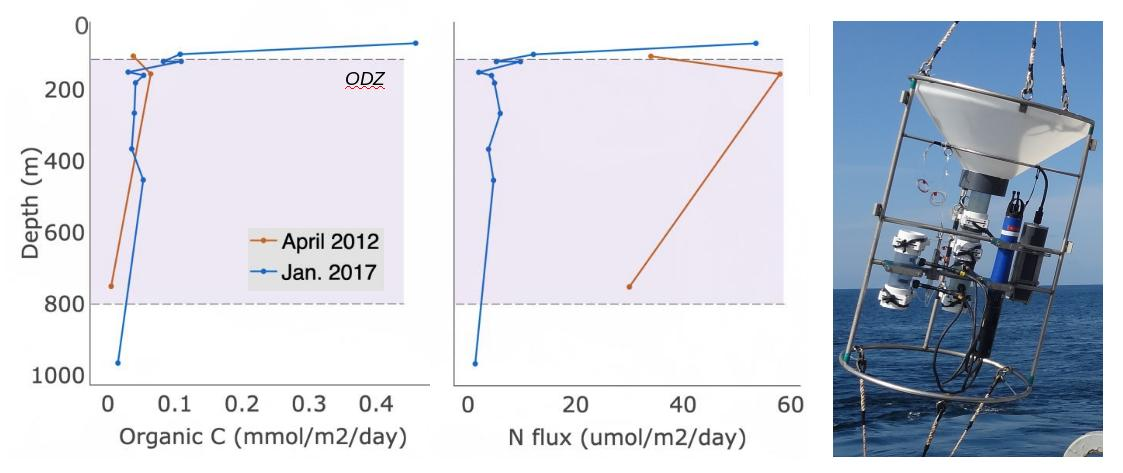
\includegraphics[width=\linewidth]{etnp-flux-trap.jpg}
	\caption{Flux profiles of organic carbon and nitrogen at offshore oligotrophic station P2 in the ETNP ODZ. The ODZ, where O\textsubscript{2} dropped below measureable quantities with a Seabird SBE 43 Dissolved Oxygen Sensor (approx. 2 $\mu$m) is shown in purple shading. \textit{Right}: a generation 5 sediment trap-incubator system.}
	\label{fig:etnp flux}
\end{figure}

Flux attenuation curves are anticipated to vary between cruise years and nearshore and offshore oligotrophic stations. All three cruises' flux samples are at UW in storage, and the 2017 suite has been processed for organic C and N by stable isotope analysis. Comparing with an earlier cruise to stations P2, the organic C and N fluxes are markedly different between April 2012 and January 2017 (Figure \ref{fig:etnp flux}). To answer \textbf{Question 3.1}, I will:

\begin{enumerate}
	\item[1.] Lead preparation of 2019 samples stable C and N isotope measurements at the UW IsoLab or UC Davis facililty (2018 samples prepared but not run).
	\item[2.] Determine attenuation coefficients or P1, P2, and P3 during all three cruises as in Keil et al., 2016 \cite{keil_multiproxy_2016}.
\end{enumerate}

\subsubsection{N\textsubscript{2} loss rate calculations from sediment trap-incubators}

My role in this field work and subsequent sample processing and data analysis is primarily the OM flux and metaproteomic work. However, key to contextualizing the OM flux and microbial processing of OM informed by metaproteomics is determining the N\textsubscript{2} loss rates due to particles. Clara Fuchsman and Allan Devol are the leads on this aspect of the project, and my contributions have been determining organic carbon and nitrogen in each incubation and amassing the metadata needed to make these calculations. 

Tracers (in this case \textsuperscript{15}NO\textsubscript{2}) were injected into the particle-concentrated and control bottles onboard the sediment traps and incubated for 4-32 hours. Once the traps are back onboard, we subsampled both chambers for \textsuperscript{30}N\textsubscript{2} and \textsuperscript{29}N\textsubscript{2} measurement by isotope ratio mass spectromtry (IRMS). Currently we have calculated N\textsubscript{2} loss rates for the 2017 cruise (1-5 nM N day\textsuperscript{-1}), which are within range of previous shipboard incubation rates at Station P2 (5-15 nM N day\textsuperscript{-1}) \cite{babbin_organic_2014}. We have prepared and are waiting only on organic carbon numbers to normalize rates from the 2018 cruises; we have not yet run samples from the 2019 cruise. To finish this project I will:

\begin{enumerate}
	\item[1.] Run 2019 incubation N\textsubscript{2} samples when normal operations resume at UW in the Stable Isotope Lab on the Delta V IRMS. 
	\item[2.] Use the \textsuperscript{29}N\textsubscript{2} and \textsuperscript{30}N\textsubscript{2}-based calculation developed by Devol et al. to determine N\textsubscript{2} loss rate over experiment. 
	\item [3.] Normalize rates to organic carbon determined by stable isotope measurements at UW IsoLab or UC Davis facilities. 
\end{enumerate}

\subsubsection{Metapeptidomic and metaproteomic signatures of POM through the ODZ}

My M.S. work focused on a subset of ETNP POM from 2017 as a first look using the \textit{de novo}-assisted peptide sequencing approach. For this project I'll expand on that work and technique to address \textbf{Question 3.3} and \textbf{Question 3.4}. \textbf{I hypothesize that in the ODZ and perhaps in the oxycline, suspended and sinking particles lead to functional diversity by creating biochemical niches for microbes that  facilitate N loss and other processes}. Metaproteomics samples (36 total) from 2017 and 2018 cruises have already been run on a Thermo Q-Exactive Plus at the UW Proteomics Resource Center. Samples come from above, within, and below the ODZ from both P1 and P2 stations. For a functional analysis of OM processing (\textbf{Question 3.3}), I will:

\begin{enumerate}
	\item[1.] Perform \textit{de novo}-assisted metaproteomics with Peaks using an assembled metagenome-derived database constructed by Clara Fuchsman, Gabrielle Rocap, and Cedar McKay.
	\item[2.] Analyze database search results using a peptide-based Gene Ontology (GO) enrichment analysis to explore community function of particles. I'll use MetaGOmics \cite{riffle_metagomics_2017}, which determines the abundance of GO functional categories by combining all GO terms associated with a peptide based on that peptide's matching database proteins. The relative abundance for each GO term is calculated by the spectral counts of the peptide. Finally, to determine the relative contribution of each taxon to a GO term, a lowest common ancestor (LCA) analysis of each peptide is performed using the top BLAST hit for the metagenome proteins containing the peptide. An example of this analysis, also investigating OM processing, can be found in Mikan et al., 2020 \cite{mikan_metaproteomics_2020}.
\end{enumerate}  

To address \textbf{Question 3.4}, I'll continue to probe both \textit{de novo} and database-identified peptides to:

\begin{enumerate}
	\item[1.] Determine quality and quantity (semi-quantitatively by spectral counts) of peptide mass modifications.
	\item[2.] Track the export of protein made by primary producers. In my preliminary look at 6 ETNP POM samples I found degraded Cyanobacterial peptides by LCA peptide analysis. This is peptide evidence of bacterial export that has been explored by other means (lipid signatures, \cite{close_export_2013}, and network analysis, \cite{richardson_small_2007}) but not in an ODZ. Figure \ref{fig:cyanomods} shows the relative numbers of peptides sequenced and identified as exclusively belonging to the phylum \textit{Cyanobacteria} in suspended and sinking particles from Station P2.
\end{enumerate}


\begin{figure}
	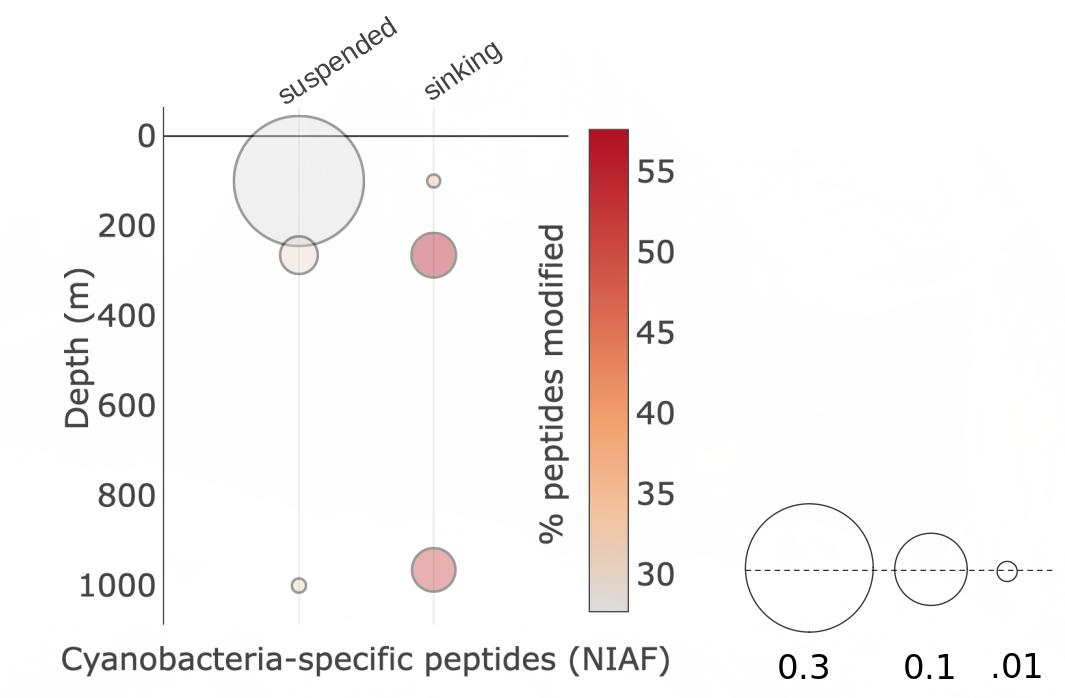
\includegraphics[width=\linewidth]{etnp2017-cyano-mods.jpg}
	\caption{Cyanobacteria-specific peptides sequenced from suspended and sinking POM from offshore Station P2, ETNP January 2017 with sampling depth. Bubble sizes represent peptide abundances scaled by the normalized ion abundance factor (NIAF) of the MS1 parent ion spectral counts. Color scale represents the percentage of peptides in each samples with mass modifications.}
	\label{fig:cyanomods}
\end{figure}

\subsubsection*{Progress}

\begin{itemize}
	\item 2017 and 2018 total mass flux samples analyzed (\textbf{Q3.1})
	\item 2017 (OC normalized) and 2018 (raw) N\textsubscript{2} loss rates calculated (\textbf{Q3.2})
	\item 2017 and (most) 2018 metaproteomics samples analyzed (\textbf{Q3.3, 3.4})
\end{itemize}


\subsubsection*{Expected outcomes}

Recent work has deconvoluted the boundaries of different water masses in the ETNP \cite{evans_role_nodate} and modeled injections of oxygen into the ODZ \cite{margolskee_ventilation_2019}. Questions of seasonality in this ODZ have given way to questions about smaller time scale variability driven by eddies, countercurrents, and subsurface zonal jets. The impacts of this variability has yet to be linked to the organic carbon cycling of the ETNP. The work of this large field project provides an extremely valuable carbon-based dataset that covers time and space in ways that can inform future modeling efforts to predict the ocean's largest ODZ. 

This continues to be highly collaborative project. I am leading the creation of a single flux, OM processing, and nitrogen loss manuscript with exact authorship to be determined. 

\subsection{Chapter 4: Organic matter exchange in the Lower Amazon River}

\subsubsection{The Lower Amazon River-to-Ocean Continuum}

The classically conceived role of rivers is that they simply export OM to the oceans and that once there, long-term preservation of terrestrially-derived OM occurs largely along continental margins. However, in recent decades rivers have come to be seen not simply as transitory pipes, but as themselves transformers and regulators that adjust the carbon cycle of not only their watersheds but also of the marine receiving waters. This paradigm shift is a result of the discovery that rivers and other inland waters outgas immense quantities of CO\textsubscript{2} and CH\textsubscript{4} to the atmosphere \cite{butman_significant_2011, richey_outgassing_2002}. 

Estimating these riverine carbon fluxes is logistically difficult, and depending on their actual magnitude, the global terrestrial CO\textsubscript{2} sink may prove to be smaller than currently estimated because rivers may mobilize and remineralize a significant component of the OM pool that is considered sequestered in soils. This poses two primary questions – \textbf{what are the geographic distributions and magnitude of aquatic CO\textsubscript{2} outgassing, and what are the dynamics that drive this outgassing?} 

The high levels of CO\textsubscript{2} supersaturation that drive gas evasion from large rivers are thought to be largely produced through \textit{in situ} respiration by heterotrophic microbes. These communities utilize OM that is fixed on land and then flushed into rivers \cite{mayorga_young_2005, ward_degradation_2013, ward_reactivity_2016}. However, there is little knowledge of what terrestrial OM compounds actually fuel this respiration or the range of their turnover rates.  Outstanding unknowns to achieving this goal are: evaluating the types of OM that are degraded in the river, their sources, the microorganisms and consortia that degrade the fixed carbon, and the metabolic pathways (aerobic, anaerobic) that lead to the large outgassing of CO\textsubscript{2} and CH\textsubscript{4}. A large team of scientists from Brazil and the U.S. led by Dr. Jeff Richey is funded to address these issues in the lower Amazon, by dar the world's largest river system by discharge, using a combination of organic geochemical and molecular biological tools.

My role in this collaboration is 1) providing a proteomic window into the microbial community processing of OM as it changes along the continuum and with hydologic conditions, and 2) characterizing the proteinaceous component of this OM along the same gradients. The primary research questions I will address are:

\bigskip

\textbf{Question 4.1} What is the microbial community composition and functioning of the lower river-to-ocean transition - what are the OM degradation pathways fueling the observed CO\textsubscript{2} exchange? Do these shift with different hydrologic regimes (high vs low water)?

\bigskip

\textbf{Question 4.2} What is the turnover of terrestrial OM (proteins, lignins, black carbon) in the river-to-ocean continuum across the different flow regimes of the year? 

\bigskip

I will address \textbf{Question 4.1} using a combination of \textit{de novo}-proteomics, underway hydrologic and gas flux measurements, and metatransciptomic analyses from previous \cite{doherty_bacterial_2017, satinsky_amazon_2014} and current collaborators. I'll address \textbf{Question 4.2} using the aforementioned techniques and datasets in addition to shipboard incubations and collaborators' geochemical measurements of lignin, black carbon, and DOM characterization by FTICR-MS.

\subsubsection{Metaproteomic insights across the Continuum}

\begin{figure}
	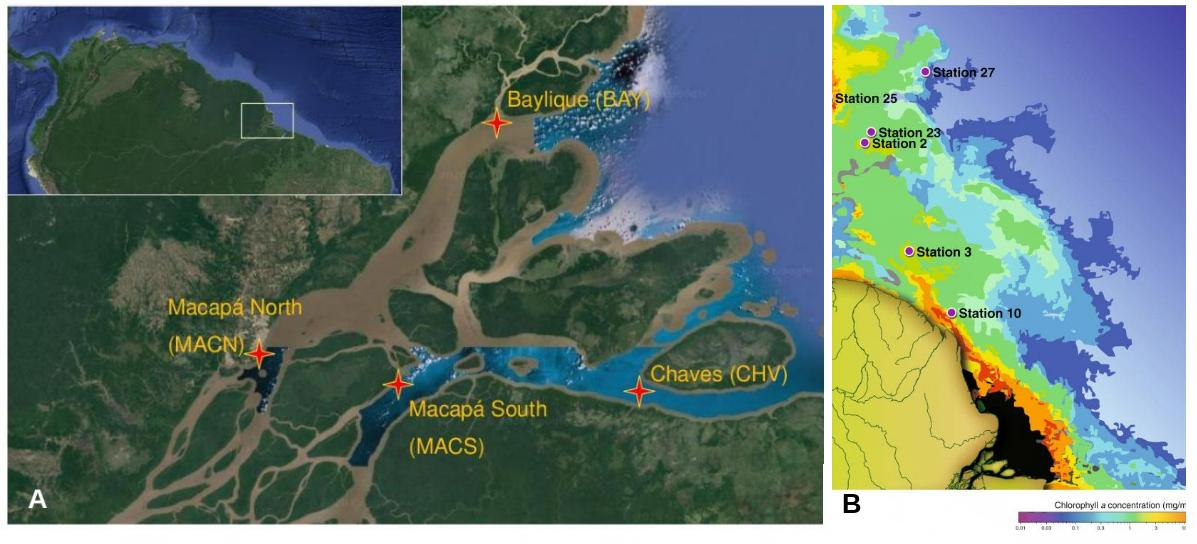
\includegraphics[width=\linewidth]{amazon-sta-map.jpg}
	\caption{A) Lower Amazon sampling stations, April 2019 on the \textit{B/M Mirage } (C) and B) stations for metagenomic and metatranscriptomic inventories of the lower Amazon river \cite{satinsky_metagenomic_2015} in May 2011 and the Amazon plume in June, 2010 \cite{satinsky_amazon_2014}. Figure adapted from Satinsky et al., 2015 \cite{satinsky_metagenomic_2015}.}
	\label{fig:amazon-stations}
\end{figure}

I've participated in one lower Amazon expedition (April 2019) and had additional samples collected by Jeff Richey in November 2019. Currently I have large suite of metaproteomics samples (approximately 200 with replicates) from 4 stations of the lower Amazon reach (Figure \ref{fig:amazon-stations}), spanning high- and low- water regimes of the hydrograph, as well as across tidal cycles. Figure \ref{fig:amazon-stations} shows the 4 stations sampled in April 2019 (at rising water) on the \textit{B/M Mirage}. Beside proteomics sampling, all four stations were sampled for DOC, DIC, alkalinity, CDOM, nutrients, and major ions. We made continuous underway measurements of pH, dissolved O\textsubscript{2}, temperature, conductivity, Chl-a, turbidity, and FDOM using YSI EXO\textsuperscript{2} sondes. Likewise, the concentration and stable isotopic composition of CO\textsubscript{2} /CH\textsubscript{4} were continuously measured. 


I plan to participate in, or get samples from, a future expedition on a boat capable of reaching further into geographic mouth and near plume (timing currently TBA). This will connect sampling from earlier Richey-led Amazon projects upriver from Macap\'{a} and genomic surveys north into the Atlantic's Amazon plume (Figure \ref{fig:amazon-stations}B). To address \textbf{Question 4.1}, I will:

\begin{enumerate}
	\item[1.] Perform \textit{de novo}-assisted metaproteomics with Peaks using an assembled metagenome-derived database constructed from published data \cite{satinsky_amazon_2014, doherty_bacterial_2017, satinsky_metagenomic_2015, ghai_metagenomics_2011}.
	\item[2.] Analyze database search results with MetaGOmics \cite{riffle_metagomics_2017}, focusing on OM processing.
	\item[3.] Compare metaproteomics results with underway CTD and gas measurements, ADCP, nutrients, C + N, and DOM (Waterhackweek project, August 2020). 
\end{enumerate}  

\bigskip

\textbf{I hypothesize that community structural and functional shifts will co-occur with changes in DOM composition.} In particular, I expect that the abundance of proteins related to specific functions (e.g. lignin degradation, primary production, and nutrient cycling) will be closely related to changes in DOM molecular formulae throughout tidal cycles, incubations, and along the study domain. I've been accepted as a participant at the UW eScience Waterhackweek workshop currently rescheduled for August 2020, where I'll bring these metaproteomic, geochemical and hydrologic datasets with the goal of synthesizing them into a searchable dataproduct. I anticipate microbial community shifts to be structured by hydrographic and tidal conditions, as has been found in Arctic rivers to the point of using genes as an accurate predictor river discharge (‘genohydrography’, \cite{good_predicting_2018}). Several other studies have established links between river flow rates and community composition \cite{crump_synchrony_2005}, including far out into the Amazon plume \cite{doherty_bacterial_2017}. 
 
\bigskip

\subsubsection{Organic matter degradation incubations}

While my goal is to enlarge the geographical lens of research in this section of the river-to-ocean domain and make to connections to pools of DOM and outgassing, I'm also interested in timescales of bacterial OM transformations and the resulting reactivity of processed material. Ward et al. \cite{ward_marine_2018} developed rotating incubation systems that better simulate river flow and particle suspension. These have been important in deciphering the source of highly reactive materials, showing that lignins, often thought to be fairly recalcitrant \cite{hedges_fluxes_1988, gough_terrestrial_1993, opsahl_distribution_1997}, are in fact remineralized in the lower Amazon. Conversely, though proteins are thought to be very labile, the mineral-laden river water may slow degradation rates due to mineral surface-protein interactions \cite{keil_sorptive_1994, mayer_relationships_1994}. For this reason, I conducted 24-hr incubations using the same rotating chambers in triplicate and paired with biochemical oxygen demand (BOD) O\textsubscript{2} respiration measurements in April 2019 at 4 stations (Figure \ref{fig:amazon-stations}) with the goal of determining protein turnover rates and contribution to heterotrophic respiration (\textbf{Question 4.2}). I plan to repeat these incubations further into the river mouth on the next field expedition, if possible. 

\subsubsection*{Progress}


\begin{enumerate}
	\item[1.] Extracted protein from the April 2019 filtered water and incubation samples in duplicate in the lab at UW in preparation for LC-HRMS when the UW Proteomics Resource Center (and campus) is open again. Protein extraction concentrations as determined by a Lowry assay show sufficient protein for analysis. 
	\item[2.] Constructed a search database from previous upriver and plume expeditions' metagenomic and metatransciptomic publications \cite{satinsky_amazon_2014, doherty_bacterial_2017, satinsky_metagenomic_2015, ghai_metagenomics_2011}(see Figure \ref{fig:amazon-stations}B).
\end{enumerate}

\subsubsection*{Expected outcomes}

This large project will likely produce several publications that will address a key knowledge gap about large rivers' carbon processing variability. My Chapter 4 publication will focus on OM processing across the study domain, looking at least at protein degradation and sources through using \textit{de novo}-assisted peptide sequencing; ideally, I will also have collaborators' dissolved black carbon, lignin, and DOM characterizations to include.  

\section{COVID-19 Considerations}

As of writing, UW Oceanography operations are proceeding remotely, with only essential work happening on campus. I have remote access to a computer to run Peaks (\textit{de novo}-assisted sequencing), and have access to all 2017 and some 2018 ETNP proteomic data, stable C and N isotope data, and metadata. All Amazon proteomics samples (April 2019 and November 2019) are in Seattle, with about 1/2 of April 2019 samples extracted but not yet run at the UW Proteomics Resource Center. 

\newpage

\section{Timeline of research}

Combined M.S./Ph.D. from September 2015 - December 2021 (6.5 years):

\begin{figure}[!htb]
	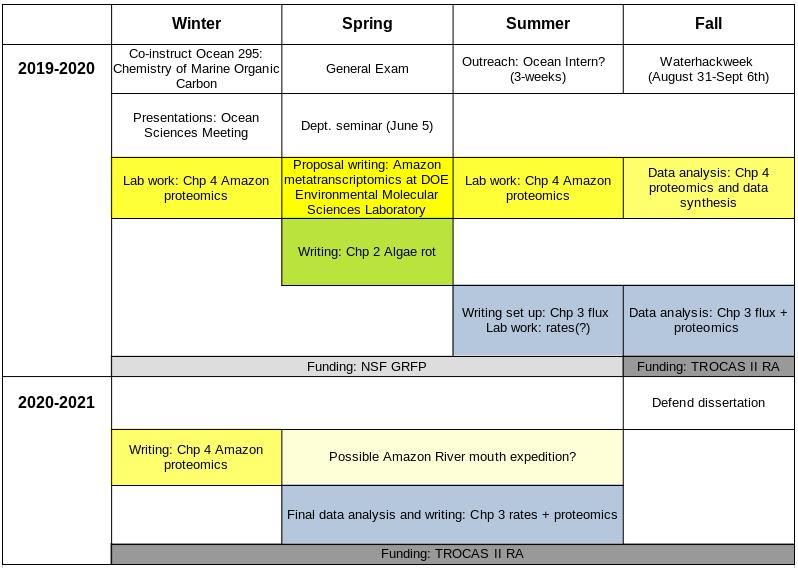
\includegraphics[width=\linewidth]{gantt.jpg}
	
	\label{timeline}
\end{figure}




\newpage

\section{References}

\printbibliography[heading=none]

\end{document}
